%!TEX root=masterproef.tex

\chapter{Implementatie}
\label{chapter:implementatie}

Voor deze masterproef werd een prototype ge\"implementeerd van de generator. Hierbij
werd FOO-lang gedefinieerd tot op het niveau dat het mogelijk was om twee
realistische voorbeelden te beschrijven. Ook de generator werd uitgewerkt tot
het niveau dat het mogelijk was om de twee voorbeelden te genereren. Zowel de
voorbeelden als de implementatie van de taal en generator zijn zo uitgewerkt
dat ze als realistische referentie kunnen dienen en dat de resultaten het
potentieel waarborgen.

Sectie \ref{section:devel-python} start dit hoofdstuk wordt met een korte
inleiding van Python, de programmeertaal die werd gekozen voor de implementatie
van het prototype.

Sectie \ref{section:devel-foo-lang} bekijkt vervolgens FOO-lang in meer detail.
Aan de hand van voorbeelden en de grammatica introduceren we de voorgestelde
taal. Een elementair voorbeeld wordt doet vervolgens dienst als rode draad
doorheen het hoofdstuk om de volledige generatie van een FOO-lang beschrijving
tot C programmacode te illustreren.

Sectie \ref{section:devel-codegen} belicht de generator met in hoofdzaak de
tweeledige hi\"erarchi van het SM en het CM. Ook het principe van
transformaties wordt kort samengevat en de onderliggende implementatie van het
\emph{visitor} patroon \citep{gamma1994design} wordt toegelicht.

De generator wordt vergezeld van gemeenschappelijke basisfunctionaliteit in de
vorm een softwarebibliotheek, genaamd FOO-lib.

Sectie \ref{section:devel-foo-lib} introduceert vervolgens de
softwarebibliotheek die de gegenereerde code vergezeld, genaamd FOO-lib. Ze
biedt toegang tot de gemeenschappelijke basisfunctionaliteit en vervangt
verschillende problematische patronen die kunnen ontstaan door slecht
gestructureerde code.

Sectie \ref{section:generation} gaat tot slot dieper in op de generatie zelf en
bekijkt het resultaat: de programmacode. 

%!TEX root=masterproef.tex

\section{Python}
\label{section:devel-python}

Als programmeertaal voor het prototype werd geopteerd voor Python, een
ge\"interpreteerde taal met dynamische typering die tevens verschillende
programmeerparadigma ondersteunt: imperatief, object-geori\"enteerd en
functioneel. Dit maakt het een zeer veelzijdige taal met veel mogelijkheden.

Python is volledig open in zijn structuur. Alles is toegankelijk en niets wordt
verborgen. Dit laat toe om elk aspect van een gegevensstructuur te manipuleren,
wat heel handig is, maar ook kan leiden tot onverwachte neveneffecten.

Alle functionaliteit, klassen of gewone functies, worden verzameld in een
\emph{module} en andere modules kunnen vervolgens deze functionaliteit
importeren. Door de volledige transparantie en dankzij introspectie, kan de
implementatie van een module zelfs dynamisch aangepast worden. Dit werd o.a.
toegepast voor het implementeren van het \emph{visitor}-patroon, in meer detail
besproken in bijlage \ref{appendix:visitor}.

Verder beschikt Python over een zeer rijke verzameling van kant-en-klare
modules, die toelaten om enkele basistaken vlot te implementeren. De
flexibiliteit en de mix van zowel imperatief als object-geori\"enteerd als
functioneel programmeren liet meermaals toe om bepaalde zaken op creatieve
manier te implementeren.

%!TEX root=masterproef.tex

\section{FOO-lang}
\label{section:devel-foo-lang}

Maar de echte belangrijke taal in dit geval is niet Python, maar FOO-lang.
Codevoorbeeld \ref{lst:hello.foo} toont de implementatie van een elementair voorbeeld
in FOO-lang. Aan de hand van dit voorbeeld introduceren we nu de typische
bouwstenen van FOO-lang en doorlopen we het hele generatieproces.

\begin{listing}[ht]
  \inputminted[linenos,frame=lines,framesep=2mm,fontsize=\footnotesize]{js}{../src/foo-lang/examples/hello.foo}
  \vspace{-3mm}
  \caption{Elementair voorbeeld in FOO-lang: \ttt{hello.foo}}
  \label{lst:hello.foo}
\end{listing}

De code start op regel 6 met de declaratie van een \emph{module}. Een module is
een op zich staand geheel en zou bv. een detectiealgoritme kunnen zijn. Alles
wat volgt op de declaratie van de module, maakt er deel van uit.

Op regel 8 introduceren we een \emph{const}ante, \ttt{interval} en stellen die
gelijk aan \ttt{1000}. Hier zien we een eerste voorbeeld van het ontbreken van
expliciete typering in FOO-lang. Dankzij type deductie zal in dit geval het
type van \ttt{interval} overeenkomen met een \emph{IntegerType}, omdat de
waarde \ttt{1000} gevormd is als een integer getal.

Ofschoon FOO-lang ge\"introduceerd wordt als DSL voor inbraakdetectie in WSN,
specificeert het zijn domein als dat van \emph{sensorknopen} of \emph{nodes}.
algoritmen met betrekking tot inbraakdetectie in WSN, hebben \'e\'en belangrijk
gemeenschappelijke entiteit en dat zijn de sensorknopen. Deze communiceren met
elkaar en op basis van die communicatie zijn zowat alle algoritmen opgebouwd.

Het concept van een knoop of \emph{node} wordt beheert door het raamwerk dat
opgebouwd wordt door de generator. De algoritmen krijgen toegang tot deze
knopen via een aantal functionele constructies. Maar ze kunnen de
basisdefinitie van een knoop in het domein uitbreiden met hun eigen
eigenschappen. Dit gebeurt bv. op regel 10, waar (de knoop van) het domein
uitgebreid wordt met een eigenschap \ttt{sequence}. Deze eigenschap wordt
expliciet getypeerd met het \emph{byte} type en krijgt als initi\"ele waarde
\ttt{0}.

FOO-lang is een \emph{functie}-geori\"enteerde taal die tracht om de functies
in de verschillende modules, zo te organiseren dat de uitvoering ervan de \mcu
of de draadloze radio zo min mogelijk belast. Op regel 14 wordt een functie
gedefinieerd, genaamd \ttt{step}. Ze accepteert \'e\'en parameter, genaamd
\ttt{node}. We merken opnieuw op dat deze parameter niet getypeerd is.

De inhoud van de functie bestaat uit programmeerconstructies die niet ongewoon
zullen overkomen en feitelijk bijna gewone C code zou kunnen zijn. Een
conditie, een eigenschap, een waardeverhoging\dots We zien hier onze eerder
toegevoegde eigenschap, \ttt{sequence}, terug opduiken.

Regel 20 brengt alle voorgaande definities nu samen in een
\emph{uitvoeringsstrategie}. FOO-lang tracht doormiddel van zijn syntax ook te
lezen als een natuurlijk taal. Indien we regel 20 gewoon lezen, zou dit iets
kunnen opleveren als ``\emph{At every (passing of) interval with nodes do (the
function named) step.}''. En dat is exact wat deze regel definieert.

In deze ene regel zien we de klassieke lus over alle gekende knopen die in
zowat alle algoritmen wel in \'e\'en of andere vorm terugkomt, echter nu is de
lus geabstraheerd tot zijn functionele betekenis.

\subsection{Syntax en grammatica}
\label{subsection:devel-foo-lang-grammar}

Het voorgaande voorbeeld gebruikt slechts een kleine subset van de volledige
mogelijkheden van FOO-lang. De volledige grammatica van FOO-lang, zoals
gedefinieerd in het kader van dit prototype, is opgenomen in bijlage
\ref{appendix:foo-lang-grammar}. Deze bijlage bevat de \emph{Extended
Backus-Naur Form} (EBNF) die de taal eenduidig bepaalt. We bespreken hier kort
enkele constructies die eerder nog niet voorkwamen.

\subsubsection{Importeren van functionaliteit}

Het is mogelijk om externe functies te importeren. Dit gebeurt aan de hand van
de constructie \ttt{from ... import ... }. Hiermee wordt een functie
ge\"importeerd vanuit een module. Zo'n module kan een andere FOO-lang module
zijn, of een extern gedefinieerde functie uit een softwarebibliotheek. In
\ref{section:devel-foo-lib} introduceren we de FOO-lib, de standaard
softwarebibliotheek die de codegeneratie vervolledigd. Hieruit worden typisch
functies geraadpleegd in de meeste beschrijvingen.

\subsubsection{Reageren op gebeurtenissen}

Naast het herhaaldelijk uitvoeren van een functie is het ook mogelijk om een
functie te koppelen aan een gebeurtenis in de context van het domein en de
knopen. In plaats van de \ttt{with ... do} constructie is het ook mogelijk om
een voor of na (\ttt{before} en \ttt{after}) de uitvoering van een functie
binnen het kader van het domein, een functie uit te voeren. Codevoorbeeld
\ref{lst:foo-event_handler} geeft een eenvoudig voorbeeld waarbij we ontvangen
berichten tellen als deze aan ons geadresseerd waren.

\begin{listing}[ht]
  \begin{minted}[linenos,frame=lines,framesep=2mm,fontsize=\footnotesize]{javascript}
after nodes receive do function(me, sender, from, hop, to, payload) {
  if(to == me) {
    me.msg_count++
  }
}
  \end{minted}
  \vspace{-5mm}
  \caption{Voorbeeld van het reageren op een gebeurtenis}
  \label{lst:foo-event_handler}
\end{listing}

In dit voorbeeld merken we ook op dat functies anoniem kunnen gedefinieerd
worden en niet eerst met een naam gedefinieerd worden.

\subsubsection{Verschillende situaties afhandelen}

Het \ttt{case statement} laat toe om eenzelfde expressie te evalueren in
verschillende situaties. Typisch gebruik voor deze constructie is het
analyseren van ontvangen gegevens. Codevoorbeeld \ref{lst:foo-case} illustreert dit.

\begin{listing}[ht]
  \begin{minted}[linenos,frame=lines,framesep=2mm,fontsize=\footnotesize]{javascript}
after nodes receive do function(me, sender, from, hop, to, payload) {
  case payload {
    contains([#marker1, value]) {
      sender.msg_sent1++
    }
    contains([#marker2, value]) {
      sender.msg_sent2++
    }
    else {
      sender.msg_other++
    }
  }
}
  \end{minted}
  \vspace{-5mm}
  \caption{Voorbeeld van het afhandelen van verschillende situaties}
  \label{lst:foo-case}
\end{listing}

In dit voorbeeld wordt de ontvangen berichten geanalyseerd en gecatalogeerd op
basis van de inhoud. Als in een berichte \ttt{\#marker1} wordt gevonden wordt
\ttt{msg\_sent1} verhoogd, in het geval van \ttt{\#marker2}, \ttt{msg\_sent2}
en anders \ttt{msg\_other}.

Dit voorbeeld introduceert tevens nog drie andere belangrijke constructies: het
\emph{atom}, lijsten en patroon koppeling.

\subsubsection{Atomen}

\emph{Atomen} werden ontleed aan Erlang. Ze stellen een uniek herkenbare
entiteit voor. Het is aan de generator met hulp van het platform en/of domein
en/of doeltaal om hiervoor een geschikte voorstelling te vinden.

In het geval van dit prototype werden twee bytes voorzien om een unieke
identificatie te maken van delen in berichten. De generator kan hier
verschillende strategie\"en volgen en beslissen op basis van de verschillende
\emph{atoms} die hij tegenkomt.

\subsubsection{Lijsten}

Lijsten worden voor verschillende doeleinden gebruikt. Ze worden syntactisch
gespecificeerd door middel van vierkante haken. Zo worden ze meestal al een
letterlijke voorstelling van de lijst opgenomen. In het voorbeeld in listing
\ref{lst:foo-case} is de \ttt{payload} parameter zo'n lijst. Ook het argument
van de \ttt{contains} methode die toegepast wordt op \ttt{payload} is een
lijst. De parameter verwacht echter niet echt een lijst, maar een patroon. In
dit geval is de lijst een deel van het patroon.

\subsubsection{Patroon koppeling}

Door middel van patronen kan er een kopping gemaakt worden tussen gegevens. In
het voorbeeld in codevoorbeeld \ref{lst:foo-case} accepteert de \ttt{contains}
methode op een \emph{lijst} een patroon. Dit patroon is een lijst en bestaat
uit variabele en niet-variabele elementen. De \ttt{contains} methode zal
trachten de niet-variabele elementen herkennen in de lijst en vervolgens bij
een succesvolle herkenning een kopping te maken tussen de variabele elementen
en de waarden in de oorspronkelijke lijst.

\subsubsection{Complexe types}

In codevoorbeeld \ref{lst:hello.foo} zagen we reeds kort een voorbeeld van typering.
De \ttt{sequence} eigenschap werd getypeerd als een \ttt{byte}. Naast
\ttt{byte} zijn er ook nog \ttt{integer}, \ttt{float}, \ttt{boolean} en
\ttt{timestamp} als standaard eenvoudige types.

Vergelijkbaar met lijsten is er ook het \emph{tuple} type. Dit zijn lijsten van
types en defini\"eren de types van de elementen van een lijst van vaste lengte.

Van alle types kan ook een veelvoud gedefinieerd worden door het toevoegen van
een \ttt{*} achter het type. Zo kunnen lijsten van een bepaald type
gedefinieerd worden. Gecombineerd met het \emph{tuple} type, ontstaat zo bv. de
mogelijkheid om lijsten van \emph{records} te defini\"eren.

In codevoorbeeld \ref{lst:foo-complex_type} wordt het \ttt{nodes} domein uitgebreid
met een \ttt{inbox} eigenschap. Deze bestaat uit meerdere \emph{tuples} die op
hun beurt bestaan uit een \ttt{timestamp} en meerdere \ttt{bytes}.

\begin{listing}[ht]
  \begin{minted}[linenos,frame=lines,framesep=2mm,fontsize=\footnotesize]{javascript}
extend nodes with {
  inbox : [timestamp, byte*]* = []
}
  \end{minted}
  \vspace{-5mm}
  \caption{Voorbeeld van een complex type}
  \label{lst:foo-complex_type}
\end{listing}

%!TEX root=masterproef.tex

\section{Code generator}
\label{section:devel-codegen}

Met FOO-lang zijn we nu in staat om inbraaddetectiealgoritmen te beschrijven.
Deze FOO-lang code moet vervolgens door de codegenerator omgezet worden in een
gewone programmeertaal. In het geval van dit prototype is dat C.

%!TEX root=masterproef.tex

\subsection{Opbouw}

Figuur \ref{fig:devel-component-overview} geeft een overzicht van de opbouw van
de oplossing.

\begin{figure}[ht]
  \centering
  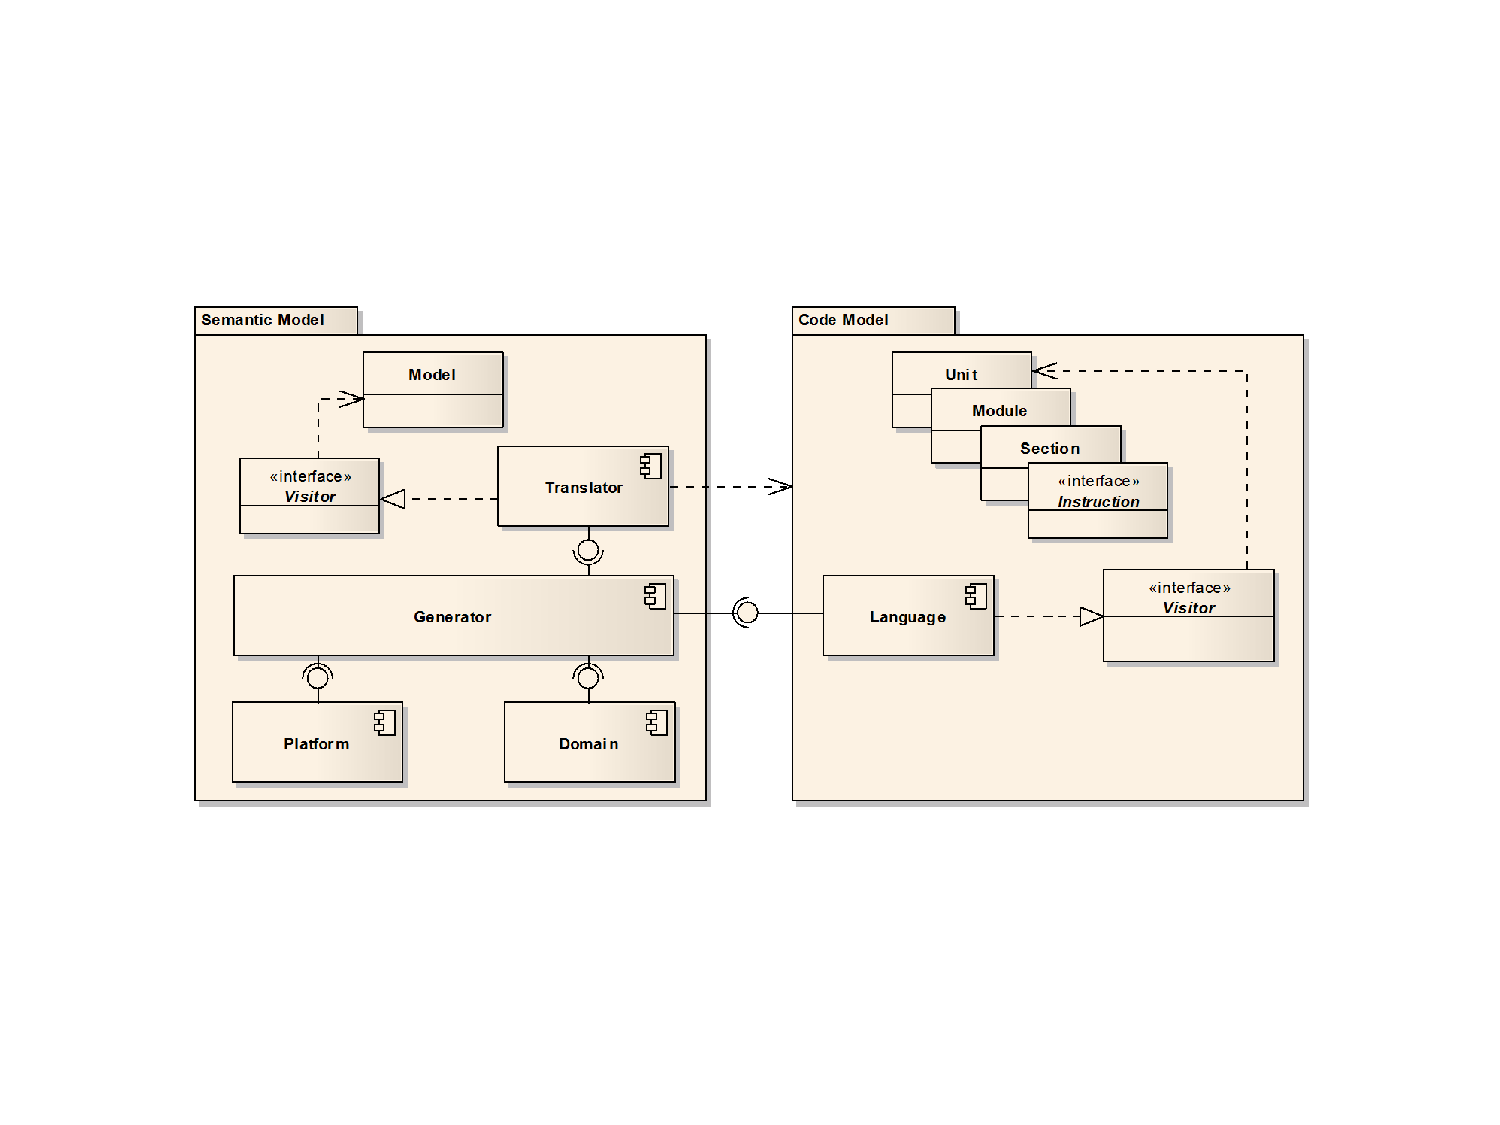
\includegraphics[width=\linewidth]{resources/component-overview.pdf}
  \caption{Overzicht van componenten en kernentiteiten}
  \label{fig:devel-component-overview}
\end{figure}

Intern bestaat de oplossing uit twee grote delen: het semantische en het
code-gedeelte. Binnen het semantische gedeelte vinden we het SM terug. Dit
model kan benaderd worden door middel van een zgn. \emph{visitor}, een
implementatie van het \emph{visitor}-patroon. Aan de hand van deze
\emph{visitor} kunnen transformaties van het model gerealiseerd worden.

Het SM is de primaire invoer voor de generator. Deze kan zijn taak slechts
vervullen door middel van een compositie met een \emph{platform-} en
\emph{domeinindefinitie}, een vertaler (\emph{Translator}) die elementen uit
het semantische gedeelte kan omzetten naar overeenkomstige elementen in het
code-gedeelte, en de uiteindelijk beoogde programmeertaal (\emph{Language}).

De programmeertaal maakt deel uit van het code-gedeelte, wat in hoofdzaakhet CM
bevat. Dit is op zijn beurt opgebouwd uit een hi\"erarchie van vier niveaus. De
structuur van de beoogde code wordt weergegeven door de compilatie \emph{unit},
de \emph{modules} en de \emph{secties}. Hier staat de unit voor het geheel, de
modules voor functioneel samenhangende delen en de secties voor een fysieke
opdeling in bestanden. De juiste realisatie van deze hi\"erarchie wordt
overgelaten aan de implementatie van de taal die hier betekenis aan kan geven.

Op het laagste niveau van het CM vinden we de \emph{instructies}. Deze kunnen
gebruikt worden om effectieve code voor te stellen. Er bestaat in het CM per
definitie een overeenkomstige instructie voor elk element uit het SM. Aangezien
het SM functioneel rijker is dan de meeste programmeertalen, moeten na
constructie van het initi\"ele CM, door middel van transformaties,
alternatieven ge\"implementeerd worden, die binnen de mogelijkheden van de
uiteindelijke programmeertaal liggen.

\subsection{ANTLR}
\label{subsection:devel-antlr}

Het generatieproces start met het inladen van de FOO-lang-bronbestanden in het
SM. Dit gebeurt door middel van een \emph{parser} die de tekstuele voorstelling
analyseert en de semantische constructies detecteert. Het resultaat van deze
stap is een boomstructuur die de betekenis van de verschillende constructies
structureel weergeeft. Zo'n boomstructuur is een AST. Figuur
\ref{fig:devel-ast} toont de AST van het elementaire voorbeeld uit
codevoorbeeld \ref{lst:hello.foo}.

\begin{figure}[ht]
  \centering
  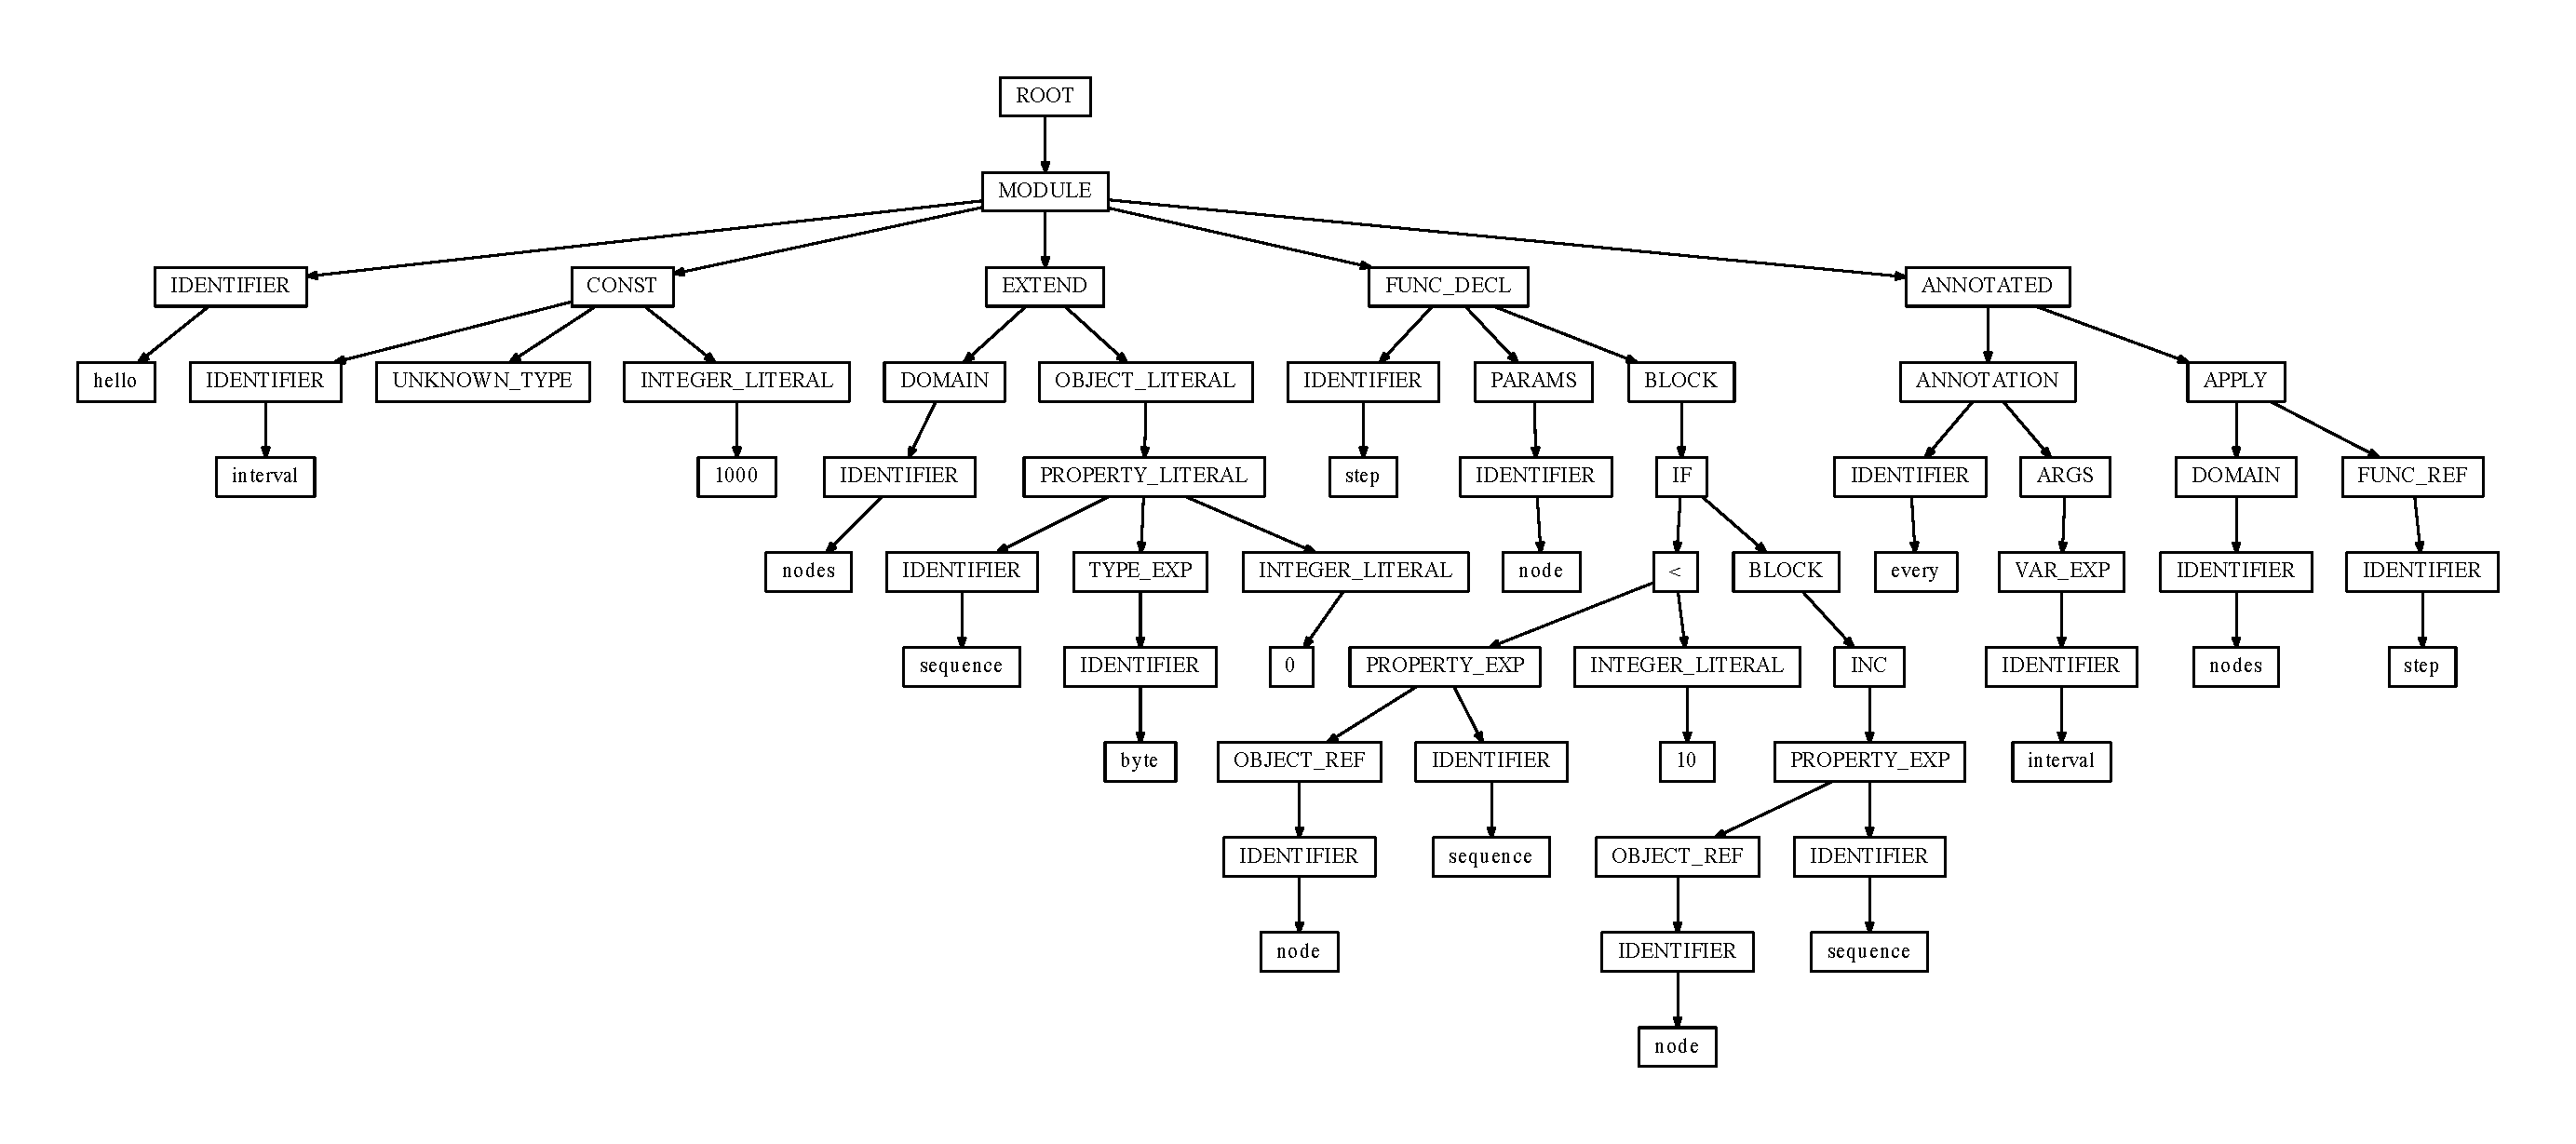
\includegraphics[width=\linewidth]{resources/hello_ast.pdf}
  \caption{De AST van het elementaire voorbeeld, \ttt{hello.foo}}
  \label{fig:devel-ast}
\end{figure}

We herkennen de inhoud van het codevoorbeeld in deze figuur: op het hoogste
niveau zien we de module met een naam (\ttt{IDENTIFIER}), de definitie van een
constante (\ttt{CONST}), een uitbreiding van het domein (\ttt{EXTEND}), een
functiedefinitie (\ttt{FUNC\_DECL}) en een geannoteerde applicatie
(\ttt{ANNOTATED}) van een functie op een domein. De AST is ontdaan van alle
ondersteunende syntax, zoals aanduidingen voor blokken code\dots en bevat
louter de semantische inhoud.

%!TEX root=masterproef.tex

\subsection{Interfaces}
\label{subsection:devel-codegen-interfaces}

Voor we het SM en het CM in detail bekijken, kijken we eerst naar de interfaces
die de codegenerator ter beschikking stelt.

\subsubsection{foo.py}

Op het hoogste niveau biedt de generator een interface via de opdrachtprompt
(\emph{Command-Line Interface}) (CLI) aan in de vorm van een Python script:
\ttt{foo.py}. Codevoorbeeld \ref{lst:foo.py-help} toont de uitvoering van het
script en geeft een overzicht van de mogelijkheden.

\begin{listing}[ht]
  \begin{minted}[linenos,frame=lines,framesep=2mm,fontsize=\footnotesize]{console}
$ source setpath.sh
$ ./foo.py --help
usage: foo.py [-h] [-v] [-c] [-i] [-g FORMAT] [-o OUTPUT] [-l LANGUAGE]
              [-p PLATFORM]
              [sources [sources ...]]

Command-line tool to interact with foo-lang and its code generation
facilities.

positional arguments:
  sources               the source files in foo-lang

optional arguments:
  -h, --help            show this help message and exit
  -v, --verbose         output info on what's happening
  -c, --check           perform model checking
  -i, --infer           perform model type inferring
  -g FORMAT, --generate FORMAT
                        output format (choices: none, ast, ast-dot, sm-dot,
                        foo, code / default: none)
  -o OUTPUT, --output OUTPUT
                        output directory (default: .)
  -l LANGUAGE, --language LANGUAGE
                        when format=code: target language (choices: c /
                        default: c)
  -p PLATFORM, --platform PLATFORM
                        when format=code: target platform (choices: moose,
                        demo / default: moose)
  \end{minted}
  \vspace{-5mm}
  \caption{Informatie over de werking van \ttt{foo.py}}
  \label{lst:foo.py-help}
\end{listing}

De CLI biedt toegang tot alle aspecten van de generator: modelcontrole
(\ttt{check}), typedeductie (\ttt{infer}), het uitvoerformaat (\ttt{format}),
plaats van de uitvoer (\ttt{output}), de programmeertaal (\ttt{language}) en
voor welk platform de generatie moet gebeuren (\ttt{platform}).

De lijst van mogelijke uitvoerformaten bestaat uit: \ttt{none}, \ttt{ast},
\ttt{ast-dot}, \ttt{sm-dot}, \ttt{foo} en \ttt{code}. Formaat \ttt{ast} toont
een hi\"erarchisch overzicht van de AST op het scherm in tekstuele vorm. De
uitvoer van \ttt{ast-dot} zagen we eerder in figuur \ref{fig:devel-ast}. De
uitvoer is code die als invoer kan dienen voor GraphViz \citep{url:graphviz},
een openbronproject dat zich specialiseert in het visualiseren van
graafgeori\"enteerde gegevens, zoals deze AST. Door middel van het
\ttt{dot}-commando kan van deze code een visuele voorstelling gemaakt worden.

Overeenkomstig bestaat er de mogelijkheid om een visuele voorstelling te maken
van het SM, door middel van het \ttt{sm-dot} formaat. Om controles te doen
betreffende de goede verwerking van de FOO-lang broncode kan een ingelezen set
van modules ook opnieuw als FOO-code uitgevoerd worden.

Tot slot is er nog het \ttt{code} formaat, dat de generator vraagt om code te
genereren. Hierbij dienen dan ook de overige opties voorzien te worden:
uitvoerlocatie, taal en platform.

\subsubsection{API}

Het \ttt{foo.py} Python-script is slechts een dunne schil rond de Python-API.
Deze biedt alle functionaliteit aan in de vorm van een Python-module met een
imperatieve interface. Codevoorbeeld \ref{lst:codegen-api} toont de interface
van deze module.

\begin{listing}[ht]
  \begin{minted}[linenos,frame=lines,framesep=2mm,fontsize=\footnotesize]{python}
def create_model():
  ...
  return model

def parse(string, noprint=False):
  ...
  return parser

def infer(model, silent=False):
  ...

def check(model, silent=False):
  ...

def generate(model, args):
  ...

def load(string, model=None):
  ...
  return model
  \end{minted}
  \vspace{-5mm}
  \caption{API van de codegenerator}
  \label{lst:codegen-api}
\end{listing}

De verschillende fasen uit het generatieproces bestaan uit het aanmaken van een
(leeg) model, het parsen van de broncode, het deduceren van onbekende types,
het controleren of een model volledig in orde is en het genereren van code. De
bijkomende \ttt{load}-functie combineert de \ttt{create\_model} en
\ttt{parse}-functionaliteit in \'e\'en handige functie.

De API laat toe om de generator vanuit Python aan te spreken en eventueel
verder te integreren in een uitgebreider compilatieproces, of om andere
interfaces te voorzien (visuele gebruikersinterfaces zoals bv. een
webinterface\dots).

Verder biedt de API toegang tot de entiteiten op het hoogste niveau, zoals de
parser, de model-entiteit uit het SM\dots De volledige openheid van Python-code
laat toe om dieper door te dringen en elk aspect van het model te ondervragen
en te wijzigen.

Beide onderliggende modellen kunnen tevens volledig benaderd worden aan de hand
van een \emph{visitor}. Deze wordt door de generator veelvuldig gebruikt, zelfs
voor kleine operaties en biedt een aantrekkelijkere interface om met de
modellen te werken dan het direct ondervragen van eigenschappen en het
aanroepen van methoden in het model.

%!TEX root=masterproef.tex

\subsection{Semantisch model}
\label{subsection:devel-semantic-model}

De AST wordt door een eerste \emph{visitor} ingeladen in het SM. Dit is in
essentie een eenvoudige vertaling van de boomstructuur naar de overeenkomstige
elementen in het SM. Het resultaat kan gevisualiseerd worden door middel van
GraphViz, zoals weergegeven in figuur \ref{fig:hello.sm}.

\begin{figure}[ht]
  \centering
  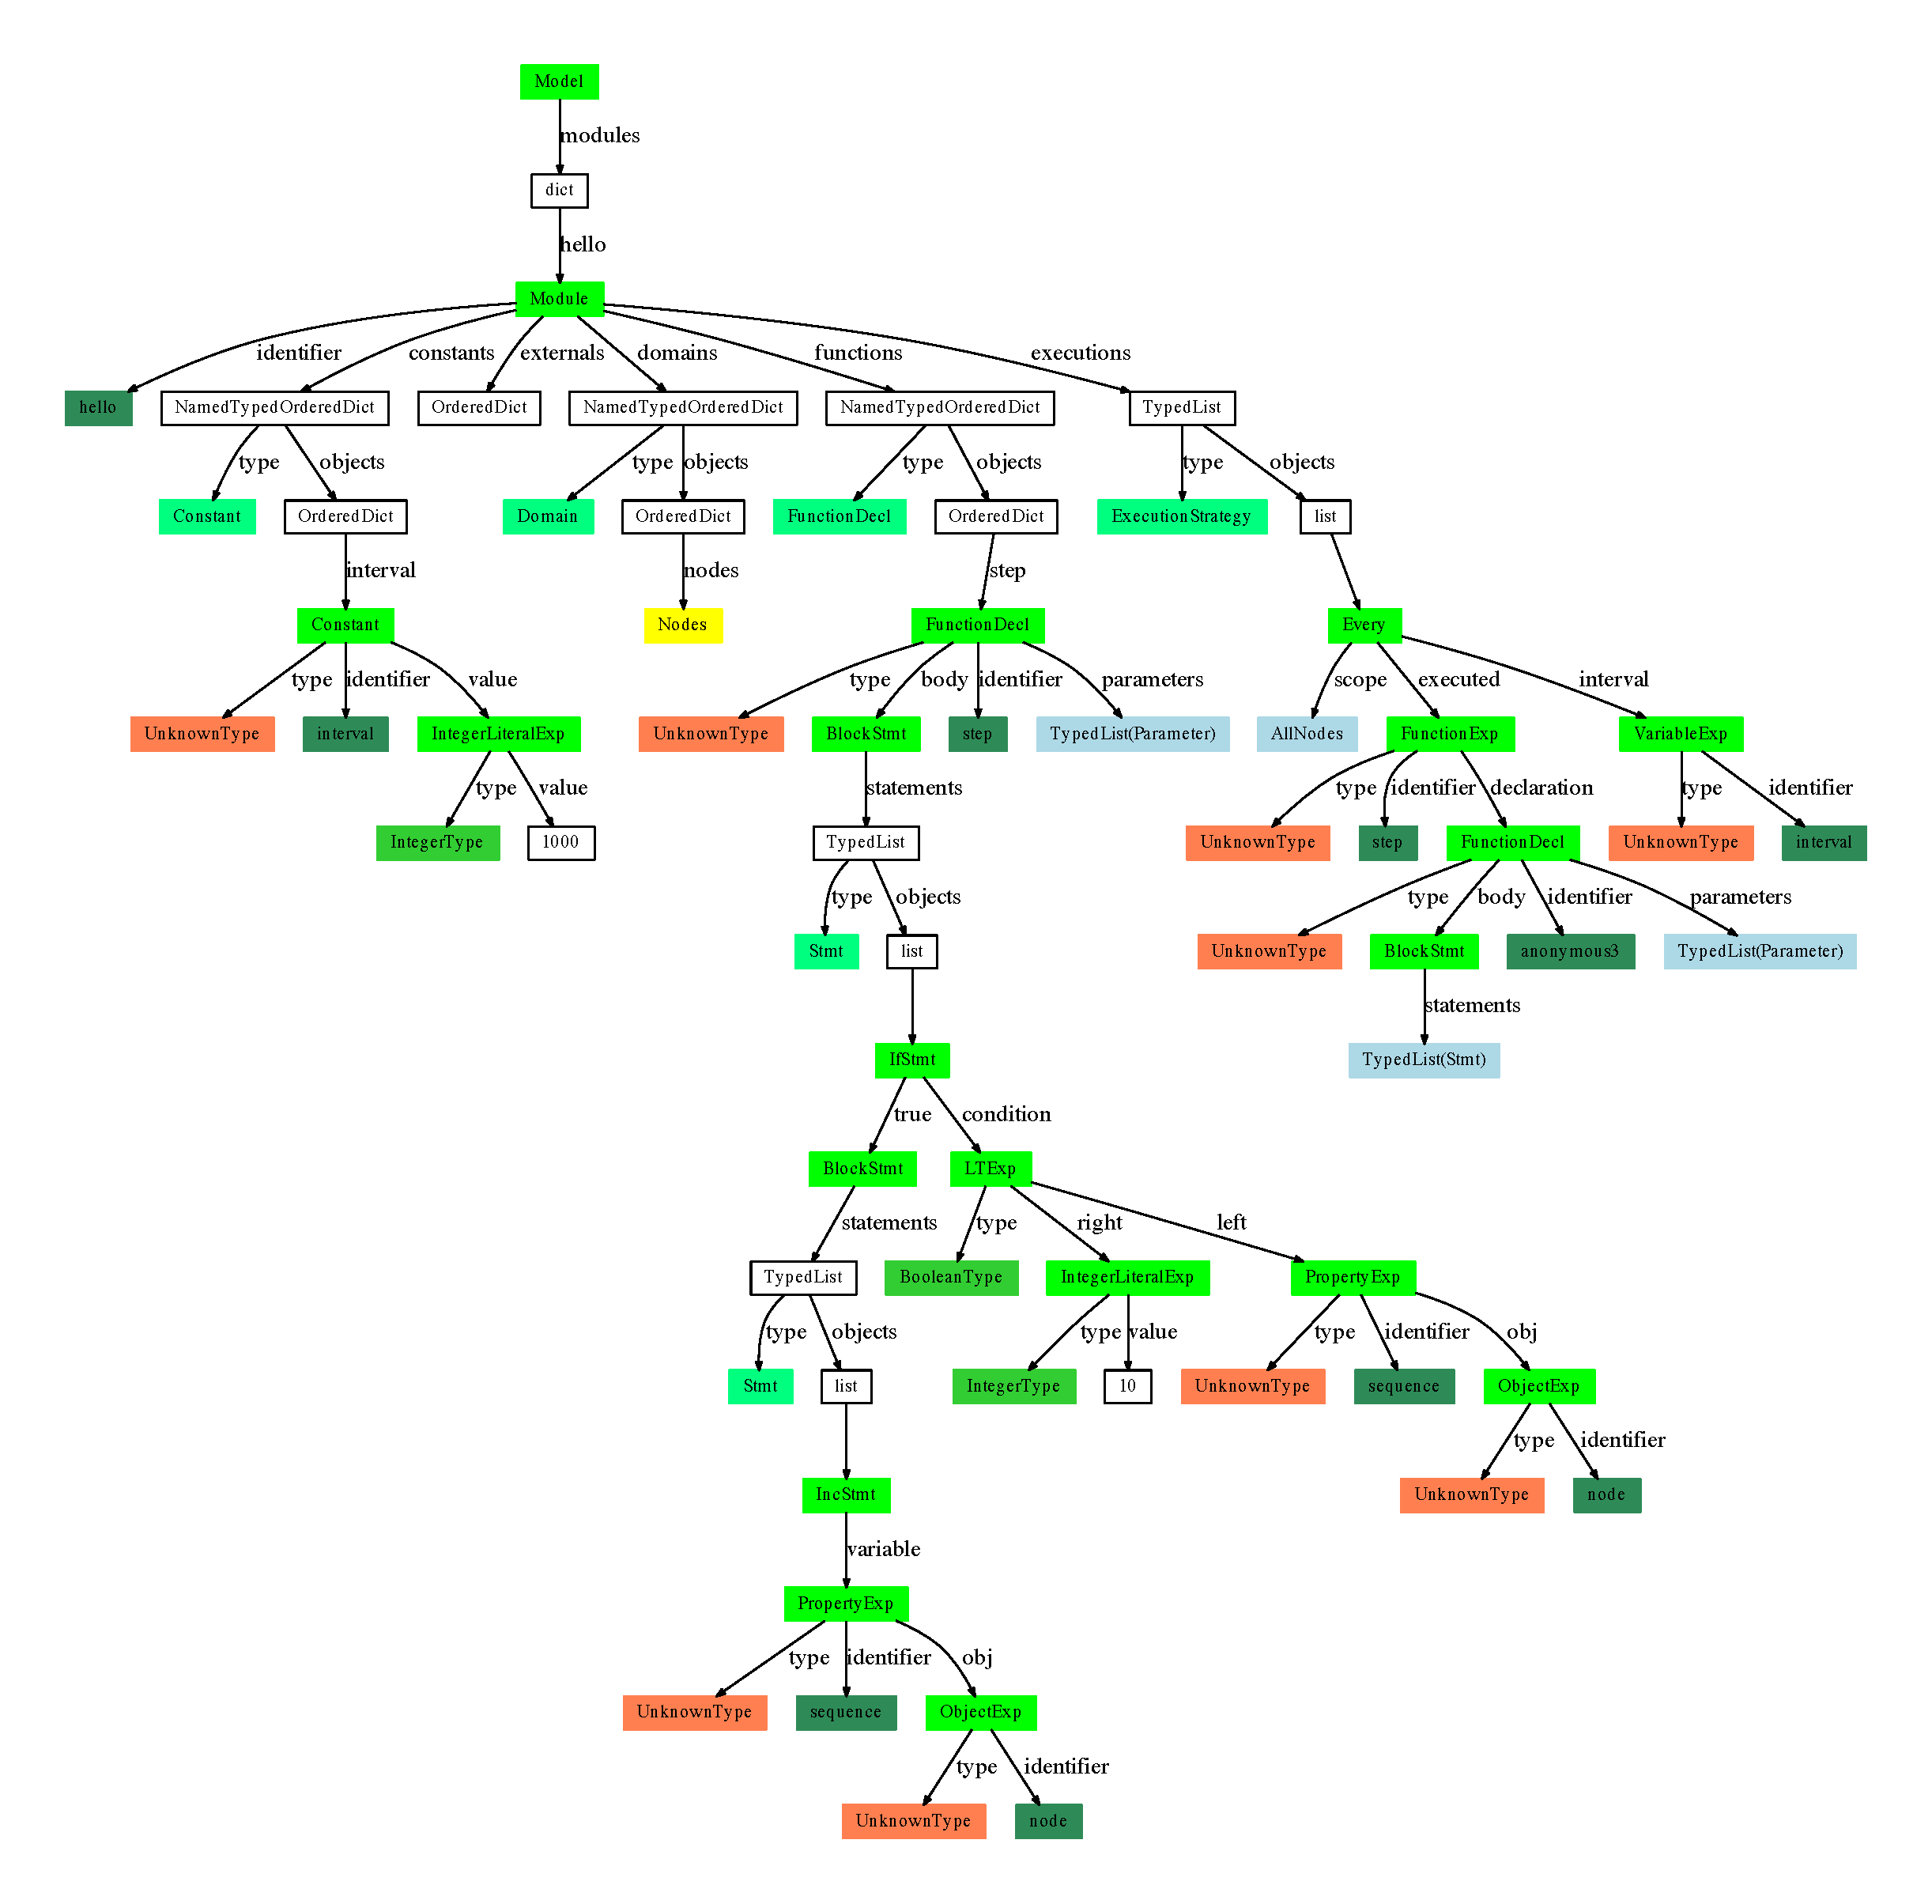
\includegraphics[width=\linewidth]{resources/hello_sm.pdf}
  \caption{Het SM van het elementaire voorbeeld, \ttt{hello.foo}}
  \label{fig:hello.sm}
\end{figure}

Het SM bevat meer informatie dan de AST, zoals bv. typering. Bij deze
visualisatie is gebruikgemaakt van een kleurencodering. Hierdoor wordt het
makkelijker om het diagram te interpreteren.

De belangrijkste kleur is zonder meer de rode kleur, die problemen in het model
aangeeft. In dit geval betreft het onbekende types. Dit is in deze fase van het
generatieproces normaal aangezien typering in FOO-lang optioneel is. Deze
eerste versie van het SM bevat daarom nog niet alle types.

Een ander deel dat lijkt te ontbreken in dit diagram is de uitbreiding van het
domein. In het voorbeeld werd immers een eigenschap \ttt{sequence} toegevoegd.
Aangezien dit een uitbreiding is van het domein, zal deze terug te vinden zijn
in de eigen instantie van het domein voor deze module. In figuur
\ref{fig:hello.sm} is dit domein beperkt tot een referentie in een gele kleur.
De volledig inhoud van wat hierachter schuil gaat, is opgenomen in bijlage
\ref{section:nodes.sm}.

Dit is een groot stuk van het SM en behelst verschillende types en
functiedeclaraties die door het \ttt{nodes}-domein ge\"introduceerd worden in
het SM. Hier vinden we tevens de uitbreiding met de extra \ttt{sequence}
eigenschap.

\vspace{-3mm}

\subsubsection{Type deductie}

De volgende stap in het generatieproces bestaat erin om de nog onbekende types
te deduceren op basis van andere informatie uit het SM. Dit gebeurt aan de hand
van de \ttt{inferrer}-module. Dit is een implementatie van de \emph{visitor}
voor het SM die nagaat of alle types gekend zijn. Voor onbekende types wordt,
afhankelijk van de plaats van het type op verschillende manieren op zoek gegaan
naar een juiste typering.

De eenvoudigste methode bouwt, terwijl het model doorlopen wordt, een overzicht
op van gekende types die ontstaan door de declaratie van variabelen\dots Indien
een onbekend type wordt gevonden, consulteert de \ttt{inferrer}-module dit
overzicht. Indien een referentie naar een eerdere declaratie gevonden wordt,
kan het type eenvoudig gededuceerd worden.

In een aantal gevallen is de deductie niet rechtstreeks af te lezen uit
declaraties en moet er naar andere mogelijke combinaties gekeken worden.
Voorbeelden hiervan zijn bv. functiedeclaraties die gebruikt worden als reactie
op een gebeurtenis. De gebeurtenis specificeert hoe de reagerende functie
gedeclareerd is. Op basis van de omkaderende gebeurtenis moet vervolgens het
overeenkomstige prototype van de functie opgezocht en gekoppeld worden.

Na het succesvol uitvoeren van deze type-deductie zijn alle voorheen onbekende
types gekend en is het model volledig. Figuur \ref{fig:hello.sm-inferred} toont
hetzelfde SM als voordien, echter nu met volledig gekende typering.

\begin{figure}[ht]
  \centering
  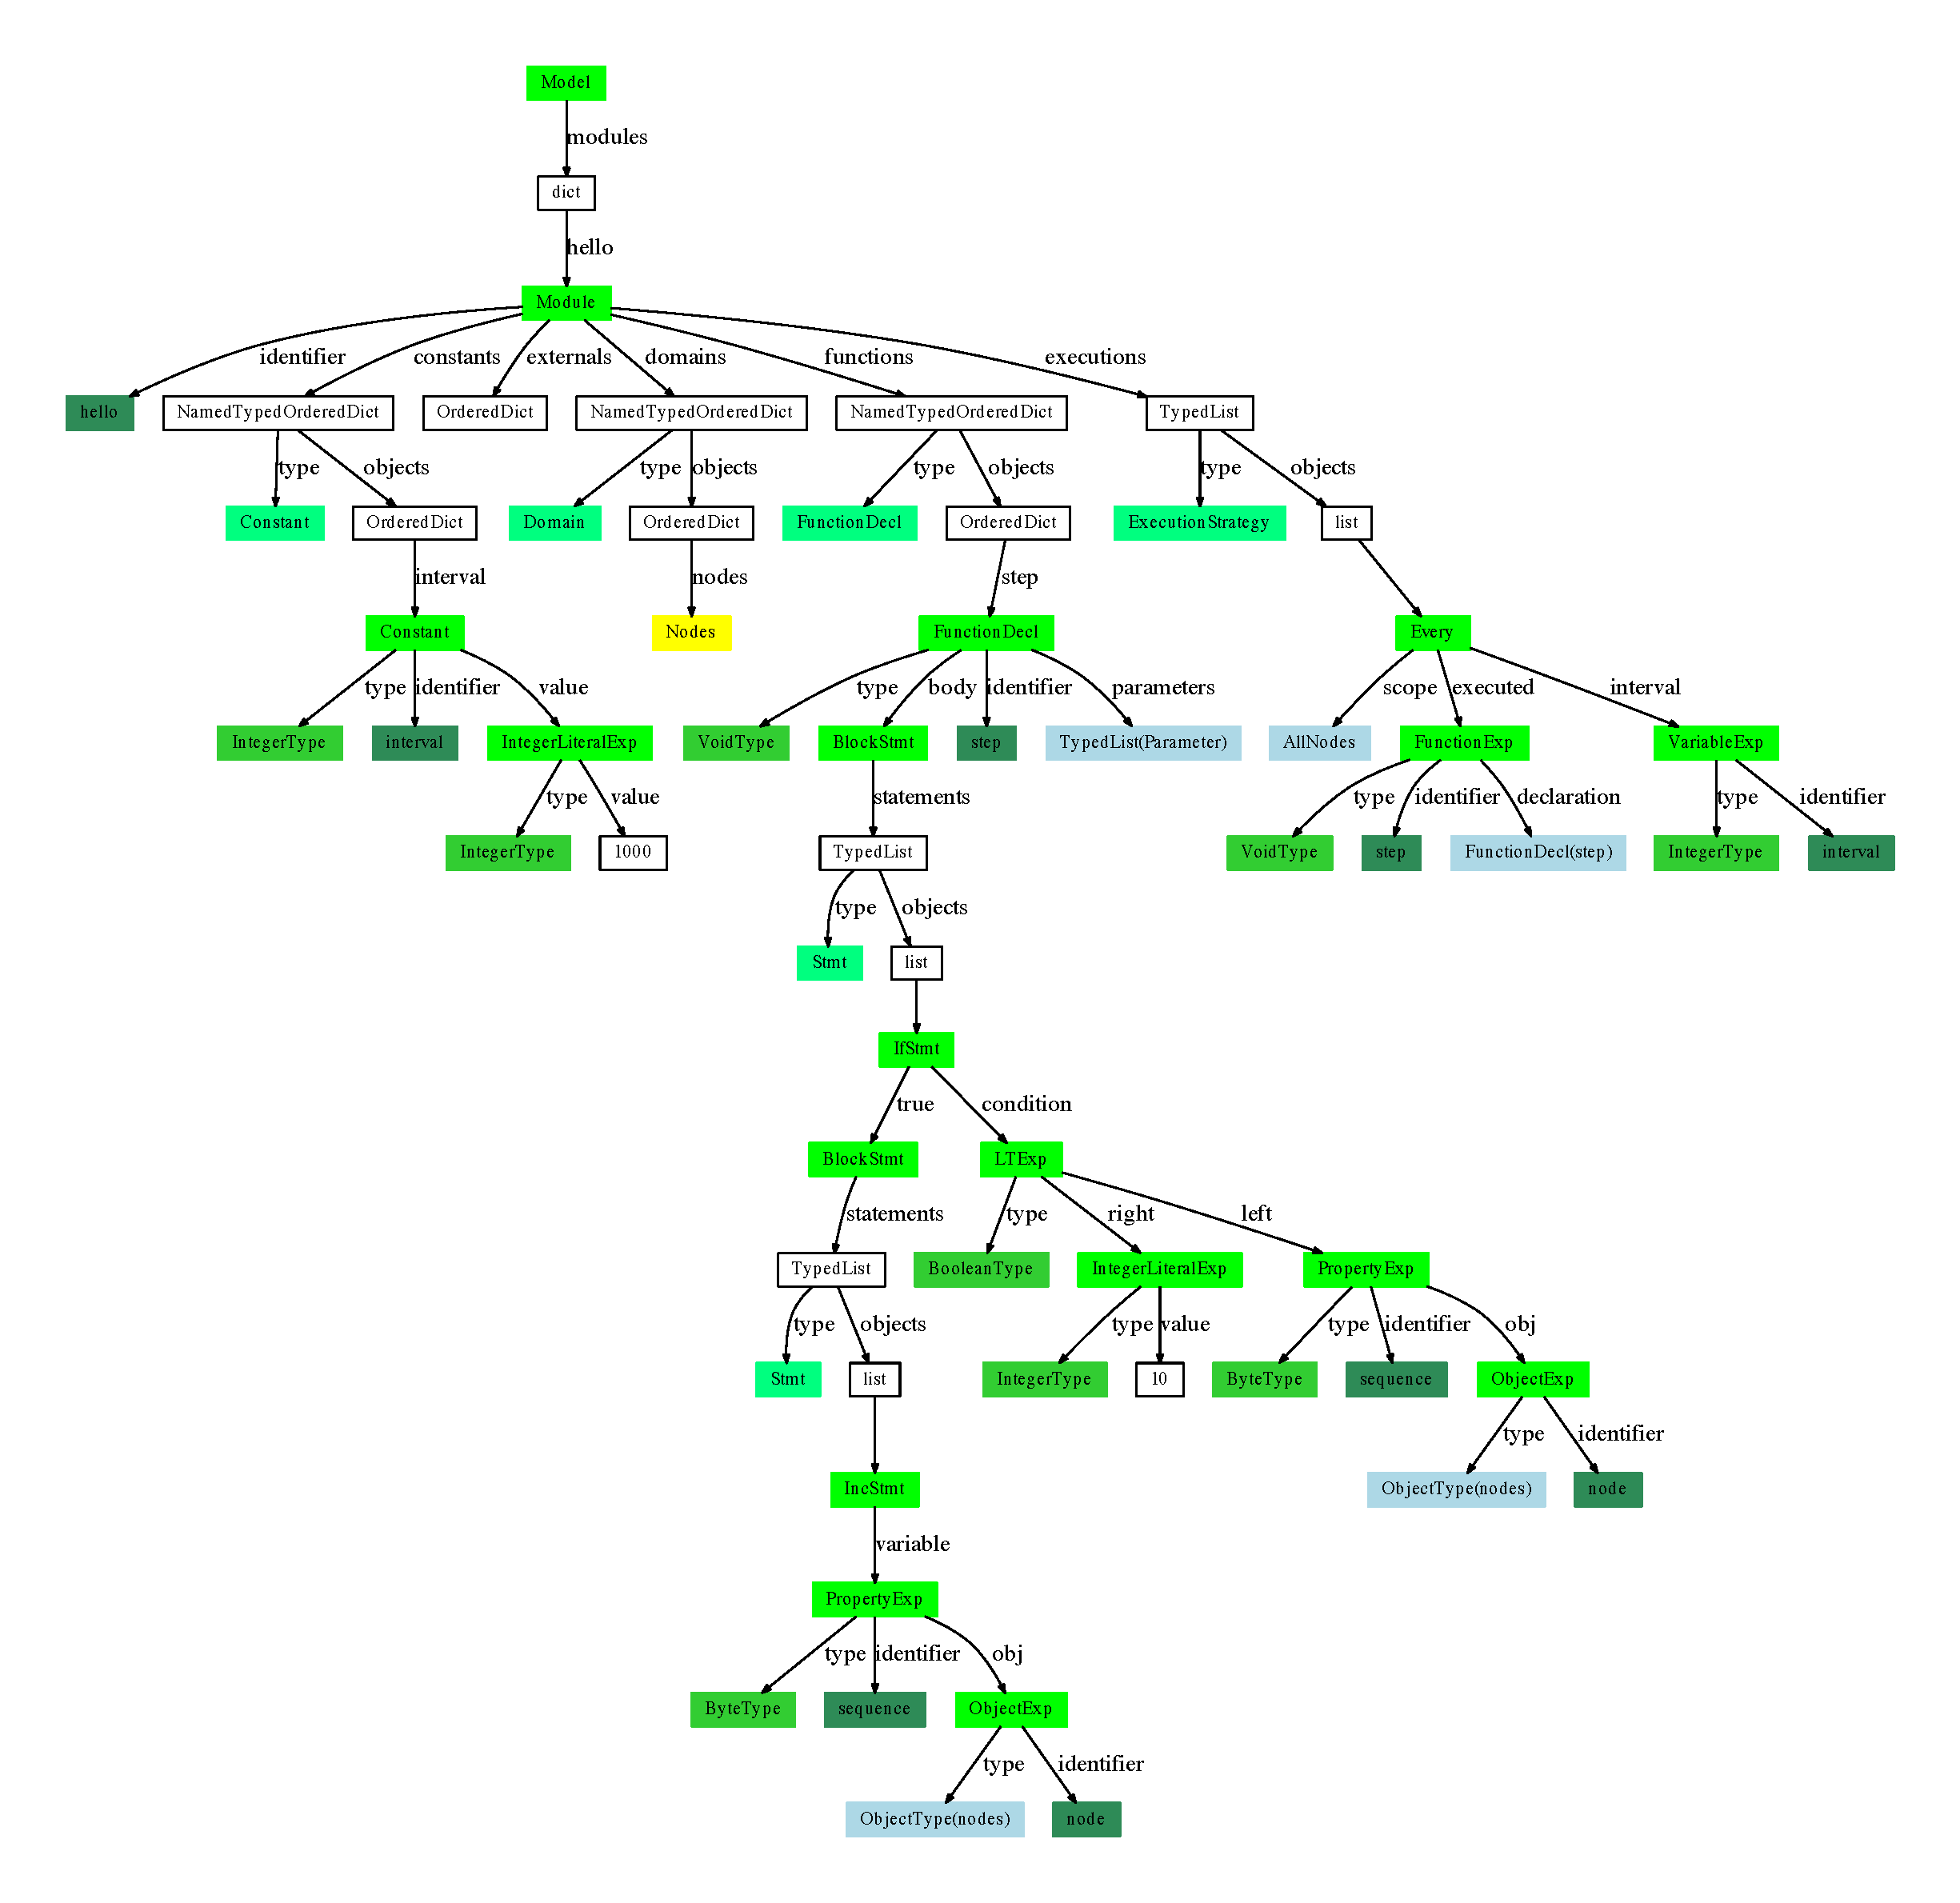
\includegraphics[width=\linewidth]{resources/hello_sm_inferred.pdf}
  \caption{Het SM van het elementaire voorbeeld, \ttt{hello.foo}, na type deductie}
  \label{fig:hello.sm-inferred}
\end{figure}

Ofschoon men verwacht dat deze fase geen structurele wijzigingen aanbrengt aan
het SM, zien we in dit geval toch dat er een vijftal elementen uit het model
verdwenen lijken te zijn. Dit is nochtans een gewoon voorbeeld van deductie. Na
het inladen van het initi\"ele model werd de (enige) uitvoeringsstrategie
gekoppeld aan een functie-expressie (\emph{FunctionExp}) genaamd \ttt{step}. Op
dat ogenblik was er over \ttt{step} niets meer geweten. De declaratie van
\ttt{step} was wel eerder gebeurd, maar het is pas in de deductiefase dat het
onbekende type van deze functie opgezocht werd. Deel van het type is tevens de
declaratie ervan. Tijdens de deductiefase wordt deze gekoppeld aan de eerdere
declaratie, waardoor in figuur \ref{fig:hello.sm-inferred} deze
functiedeclaratie niet meer volledig getoond wordt, maar nu als een referentie
naar de \ttt{step} functie opgenomen is.

\vspace{-3mm}

\subsubsection{Model controle}

De \ttt{inferrer}-module tracht alle onbekende types te deduceren. Een tweede
ondersteunende module is de \ttt{checker}-module of modelcontrole. Deze
overloopt aan de hand van een \emph{visitor} het hele model en controleert of
alles in orde is.

De \ttt{checker}-module is typisch nuttig bij het schrijven van FOO-lang code
en kan dienen als syntactische en semantische controle. Wanneer er bv. een
schrijffout gemaakt wordt in de naam van een variabele of functie, kan dit soms
niet direct opvallen. FOO-lang maakt bv. automatisch declaraties voor
variabelen aan wanneer zij voor het eerst gebruikt worden en nog niet eerder
gedeclareerd werden. De \ttt{checker}-module kan bv. voor deze situaties
waarschuwingen geven, die kunnen helpen bij het schrijven van de FOO-lang
broncode.

%!TEX root=masterproef.tex

\subsection{Code model}
\label{subsection:devel-code-model}

Het CM staat in feite volledig los van de generator en het SM en is ook als een
op zich staand project ontwikkeld als generieke beschrijving van uitvoerbare
code, genaamd \emph{CodeCanvas}.

\subsubsection{CodeCanvas}

CodeCanvas biedt een API om hi\"erarchische structuren te bouwen. Deze kunnen
opgebouwd worden uit zelf te defini\"eren entiteiten bestaan. Standaard
voorziet CodeCanvas de concepten \emph{unit}, \emph{module} en \emph{sectie}.

Een \emph{unit} is het hoogste niveau en verzamelt alle onderliggende
\emph{modules}. Een \emph{module} komt overeen met een functioneel geheel en
bestaat standaard uit twee \emph{secties}, \'e\'en voor declaraties en \'e\'en
voor definities. Een \emph{sectie} kan verder ingevuld worden met \emph{code
instructies}.

Daarnaast biedt CodeCanvas de mogelijkheid om entiteiten te markeren met een
label (\emph{tag}) en onderliggende entiteiten te selecteren of zoeken
op basis van die labels.

Dankzij een \emph{vloeiende} (\emph{fluent}) interface laat CodeCanvas
toe om zeer leesbare operaties te formuleren op deze hi\"erarchische
codestructuren.

Codevoorbeeld \ref{lst:codecanvas-hello} toont een eenvoudig voorbeeld dat de
meeste functionaliteit toepast. 

\begin{listing}[ht]
  \begin{minted}[linenos,frame=lines,framesep=2mm,fontsize=\footnotesize]{python}
from structure import Unit, Module
import instructions as code
import languages.C  as C

unit = Unit().append( Module("hello") )
main = unit.select("hello", "dec").append(code.Function(name="main"))
main.append(code.Print("Hello World\n"))

print str(unit)
print C.Emitter().emit(unit)
print str(unit)
  \end{minted}
  \vspace{-5mm}
  \caption{Werking van het \emph{CodeCanvas}}
  \label{lst:codecanvas-hello}
\end{listing}

Het voorbeeld construeert op regel 5 een \emph{unit} aan en voegt er een
\emph{module} genaamd \ttt{hello} aan toe. Achterliggend worden bij de aanmaak
van een module onmiddellijk 2 \emph{secties} toegevoegd, genaamd \ttt{dec} en
\ttt{def}.

Op regel 6 wordt vertrekkende van de \emph{unit} de \ttt{dec} \emph{sectie}
geselecteerd. De \ttt{select} methode laat toe om een opeenvolgende reeks van
\emph{labels} te defini\"eren die het pad vormen vanaf de startentiteit tot de
te selecteren entiteit.

Een gelijkaardige methode, \ttt{find}, accepteert ook een variabele lijst
argumenten en zoekt vervolgens, vertrekkende van de startentiteit, naar
entiteiten die alle opgegeven \emph{labels} dragen.

Beide methodes kunnen lijsten van entiteiten teruggeven. Op deze lijsten kunnen
evengoed alle methoden opgeroepen worden als op een enkele entiteit. Dit
resulteert in een zeer transparante interface.

De geselecteerde sectie wordt vervolgens een functie toegevoegd met de naam
\ttt{main}. Op regel 7 wordt aan deze functie een \ttt{print} opdracht
toegevoegd. Tot slot wordt de \emph{unit} op twee manieren uitgevoerd: eerst
door er een tekstuele voorstelling van te maken en in tweede instantie door
gebruik te maken van een programmeertaal, in dit geval C.

De uitvoer van dit programma is weergegeven in \ref{lst:codecanvas-output} en
toont eerst de technische tekstuele voorstelling van de hi\"erarchie. Tussen
vierkante haakjes staan de \emph{labels} die aan een entiteit verbonden zijn.
Effectieve instructie-implementaties tonen hun parameters als een verzameling
van de naam en de waarde.

\begin{listing}[ht]
  \begin{minted}[linenos,frame=lines,framesep=2mm,fontsize=\footnotesize]{console}
  Module hello [hello]
    Section def [def]
    Section dec [dec]
      Function {'params': (), 'type': void, 'id': main}
        Print {'args': (), 'string': "Hello World\n"}

  void main(void);
  #import <stdio.h>
  void main(void) {
    printf("Hello World\n");
  }
  
  Module hello [hello]
    Section def [def]
      Prototype {'params': [], 'type': void, 'id': main}
    Section dec [dec]
      Import {'imported': '<stdio.h>'} [import_stdio] <sticky>
      Function {'params': [], 'type': void, 'id': main}
        Print {'args': (), 'string': "Hello World\n"}
  \end{minted}
  \vspace{-5mm}
  \caption{Uitvoer van voorbeeld werking van het \emph{CodeCanvas}}
  \label{lst:codecanvas-output}
\end{listing}

Het tweede deel van de uitvoer toont de overeenkomstige C code voor deze
hi\"erarchie. We merken hier op dat op regel 7 een prototype en op regel 8 een
\emph{import} opdracht verschijnen die niet in de hi\"erarchie voorkwamen.

Wanneer we een tweede maal de \emph{unit} omvormen tot een tekstuele
voorstelling, zien we deze twee entiteiten wel opduiken. De uitvoermodule voor
de C programmeertaal werkt in meerdere stappen. 

Tijdens een eerste fase wordt de hi\"erarchie doorlopen en worden uitbreidingen
gedaan. In dit voorbeeld gebeuren er twee: wanneer een \emph{print} opdracht
gevonden wordt, wordt een \emph{import} opdracht toegevoegd die de declaraties
van \ttt{stdio.h} zal inladen. Een tweede transformatie zal voor elke
\emph{functie} een prototype aanmaken in de declaratie sectie van de module.

Deze fase zorgt ook voor het omzetten van constructies die niet standaard
ondersteund worden naar uitwerkingen met constructies die wel bestaan bij de
beoogde taal. Een voorbeeld hiervan zijn bv. \emph{tuples}. Deze worden door de
omvormer van C herschreven door middel van structuren en functies om deze
structuren te benaderen en onderhouden.

In een tweede fase doorloopt de uitvoermodule opnieuw de volledige
hi\"erarchie, maar vormt nu elke entiteit om in de overeenkomstige tekstuele C
syntax.

Beide fasen worden ge\"implementeerd door middel van \emph{visitors}. Deze
\emph{visitor} is tevens beschikbaar van buitenaf en laat toe om andere
transformaties te implementeren.

\subsubsection{Filosofie}

De doelstelling van CodeCanvas is het aanbieden van een API die toelaat om te
werken zoals zoals programmeur denkt/werkt tijdens programmeren, maar nu op
basis van een abstracte programmeertaal die een superset aanbiedt van
constructies uit verschillende programmeertalen.

Enkele typische eigenschappen die deze doelstelling ondersteunen zijn:

\begin{description}

  \item[Functionele cross-referenties] - Door middel van \emph{labels} en de
  \emph{selectie} en \emph{zoek} functionaliteit kan er op functionele wijze
  omgegaan worden met code. Zo kan een gebruiker een in de beschrijving van een
  functie een \emph{label} toevoegen en hier later eenvoudig naar verwijzen om
  nog bijkomende logica toe te voegen.

  \item[Zoek-en-wijzig] - Dankzij de functionele cross-referenties en de
  transparantie van een enkele entiteit of een lijst van entiteiten is het heel
  eenvoudig om algemene aanpassingen door te voeren. Dit kan bv. gebruikt
  worden om aan het begin van alle declaratie-secties een standaard blok
  commentaar te plaatsen of om systematisch aanpassingen met betrekking tot
  naamgeving door te voeren.

  \item[Automatische vervolledigen] - Het voorbeeld van het automatisch
  toevoegen van \ttt{import} opdrachten of \ttt{prototypes} bieden een
  krachtige manier om de gebruiker te ontslaan van redundant en repetitief werk.

\end{description}

%!TEX root=masterproef.tex

\subsection{Transformaties}
\label{subsection:transformations}

\TODO

\subsubsection{Het visitor patroon}
\label{subsubsection:devel-visitor-pattern}

\TODO


%!TEX root=masterproef.tex

\section{FOO-lib}
\label{section:devel-foo-lib}

\TODO

%!TEX root=masterproef.tex

\section{Generatie}
\label{section:generation}

Alle voorgaande structurele componenten zorgen samen voor het generatieproces.
Dit proces accepteert FOO-lang broncode, importeert die in het SM,
transformeert die in een CM en uiteindelijk wordt dat CM uitgevoerd als
effectieve programmacode.

Bijlage \ref{appendix:hello-srcs} bevat de belangrijkste gegenereerde code voor
het elementaire voorbeeld, \ttt{hello.foo}. We overlopen enkele aspecten van
deze laatste stap in het generatieproces en tonen hoe de verschillende
componenten bijdragen tot bepaalde van de patroonmatige constructies.

\subsection{main.c}

Deze platform-implementatie gaat uit van de eenvoudigste opzet, op basis van
een expliciete \emph{event loop} (regels 18 tot 24). Verder voorziet de
generatie aan de hand van commentaar enkele instructies voor de gebruiker om
applicatie-specifieke code toe te voegen of om het gebruikte onderliggende
raamwerk te initialiseren (zie respectievelijk regels 9 en 4 in de broncode van
\ttt{main.c}).

We merken vooral de functie-oproepen op naar functies met een
``\ttt{nodes\_}''-prefix. Deze gaan naar de \ttt{nodes} knoopgeori\"enteerde
module die deel uitmaakt van de FOO-lib softwarebibliotheek. Op regel 28 zien
we bv. de registratie van de uitvoerstrategie die na het verstrijken van een
intervaltijd telkens de functie \ttt{step} zal oproepen.

Die \ttt{interval} constante is gedefinieerd in het \ttt{constants.h} bestand,
samen met eventueel andere constanten. De generator tracht om functioneel
verwante zaken bij elkaar te plaatsen. Zo gaan dus alle constanten in \'e\'en
bestand, maar ook het importeren van functionaliteit wordt gecentraliseerd om
de te genereren code eenvoudiger te maken. Zo worden bv. alle nodig
\emph{\#include} opdrachten ook in \'e\'en \ttt{includes.h} bestand
samengebracht.

\subsection{node\_t.h en node\_t.c}

H\'et centrale gegeven is natuurlijk de voorstelling van een sensorknoop. De
generator zal de informatie uit verschillende FOO-lang modules trachten samen
te brengen tot \'e\'en gemeenschappelijk voorstelling.

Standaard heeft een knoop twee eigenschappen, nodig voor de interne werking van
de \ttt{nodes} module: een unieke, interne identificatie (\ttt{id}) en het
netwerkadres van de knoop (\ttt{address}). Daarnaast voegt de generator alle
uitgebreide eigenschappen toe en maakt van het geheel een structuur en een
\ttt{node\_t} type.

Naast de declaratie van het type, wordt ook een functie voorzien om een nieuwe
knoop te initialiseren. Deze functie bevat opdrachten die overeenkomen met de
gedefinieerde initi\"ele waarden van de eigenschappen.

\subsection{nodes-\emph{module}.h en nodes-\emph{module}.c}

Tot slot zal de generator het \ttt{nodes} domein de kans bieden om voor elke
FOO-lang module een CM module te maken. Hierin wordt de functionaliteit die
eigen is aan de module ondergebracht. Typisch vinden we hier de functies terug
die eerder gekoppeld werden aan een uitvoerstrategie.

In het geval van het voorbeeld is dit de \ttt{step} functie.

\subsection{Communicatie}

Aan het elementaire voorbeeld ontbreekt natuurlijk \'e\'en heel belangrijk
aspect: communicatie. Er worden geen berichten verstuurd, noch ontvangen. De
generator zal het versturen van berichten delegeren naar de \ttt{nodes} FOO-lib
module en zal voor het verwerken van ontvangen berichten functies registreren
bij diezelfde module. Deze worden vervolgens opgeroepen indien een binnenkomend
bericht voldoet aan de eisen voor die specifieke verwerkingsfunctie.

Codevoorbeelden \ref{lst:comm.foo} en \ref{lst:comm.c} illustreren het typische
communicatiepatroon en de overeenkomstige generatie.

\begin{listing}[ht]
  \begin{minted}[linenos,frame=lines,framesep=2mm,fontsize=\footnotesize]{javascript}
after nodes receive do function(me, sender, from, hop, to, payload) {
  // payload is a list of data. we can consider one or more cases
  case payload {
    // e.g. we can check if we find an atom and three variables after is
    contains( [ #heartbeat, time:timestamp, sequence, signature:byte[20] ] ) {
      ...
    }
  }
}
  \end{minted}
  \vspace{-5mm}
  \caption{Verwerking van een binnenkomend bericht in FOO-lang}
  \label{lst:comm.foo}
\end{listing}

Via een uitvoerstrategie wordt een (anonieme) functie gekoppeld aan het
ontvangen van een bericht door een knoop. Vervolgens wordt gecontroleerd op
verschillende mogelijke patronen. Een bericht dat een \ttt{\#heartbeat}
\emph{atoom} bevat, zal de volgende bytes koppelen aan drie variabelen:
\ttt{time}, \ttt{sequence} en \ttt{signature}.

\begin{listing}[ht]
  \begin{minted}[linenos,frame=lines,framesep=2mm,fontsize=\footnotesize]{c}
void init(void) {
  ...
  payload_parser_register(nodes_process_incoming_case_0, 2, 0x00, 0x01);
  ...
}
...
void nodes_process_incoming_case_0(node_t* me, node_t* sender, node_t* from,
                                   node_t* hop, node_t* to, payload_t* payload) {
  // extract variables from payload
  uint32_t time = payload_parser_consume_timestamp();
  uint8_t sequence = payload_parser_consume_byte();
  uint8_t* signature = payload_parser_consume_bytes(20);
  ...
}
  \end{minted}
  \vspace{-5mm}
  \caption{Gegenereerde code voor een binnenkomend bericht}
  \label{lst:comm.c}
\end{listing}

De generator zal de verwerking van een binnenkomend bericht detecteren en dit
uit elkaar halen en structureren aan de hand van een functie en een registratie
van die functie.

Het \emph{atoom} is hier omgezet in twee opeenvolgende bytes: \ttt{0x00, 0x01}.
Wanneer de algemene parser deze sequentie ontmoet, zal
\ttt{nodes\_process\_incoming\_case\_0} opgeroepen worden. De signatuur van
deze functie bevat alle informatie over het bericht ivm afzender,
bestemmeling\dots

Het vervolg van het gezochte patroon vinden we hier tevens terug. De drie
variabelen worden gedeclareerd en ge\"initialiseerd door middel van een aantal
functies die de volgende bytes uit het bericht zullen omzetten naar een
gewenste voorstelling.

\subsection{\emph{Tuples}, lijsten en meer patroonherkenning}

Net zoals het \ttt{node\_t} type, worden voor \emph{tuples} ook structuren
aangemaakt en functies gegenereerd die de behandeling van het \emph{tuple}-type
toelaten. Alle declaraties van de types en de definities van de manipulerende
functies worden samengebracht in respectievelijk \ttt{tuples.h} en
\ttt{tuples.c}. Codevoorbeeld \ref{lst:tuples.h} toont de typische module
interface van een gegenereerd \emph{tuple}.

\begin{listing}[ht]
  \begin{minted}[linenos,frame=lines,framesep=2mm,fontsize=\footnotesize]{c}
typedef struct tuple_0_t {
  uint32_t elem_0;
  payload_t* elem_1;
  struct tuple_0_t* next;
} tuple_0_t;
tuple_0_t* make_tuple_0_t(uint32_t elem_0, payload_t* elem_1);
void free_tuple_0_t(tuple_0_t* tuple);
tuple_0_t* copy_tuple_0_t(tuple_0_t* source);
  \end{minted}
  \vspace{-5mm}
  \caption{Gegenereerde code voor een \emph{tuple}}
  \label{lst:tuples.h}
\end{listing}

Aangezien een \emph{tuple} in FOO-lang gedefinieerd wordt op basis van types,
worden standaardnamen gebruikt voor de elementen. Tevens voorziet een
verwijzing naar zichzelf, om de constructie van lijsten toe te laten. Drie
functies bieden de mogelijkheid om een \emph{tuple} aan te maken, vrij te geven
of te kopi\"eren.

\emph{Tuples} worden meestal in combinatie met lijsten gebruikt. Codevoorbeeld
\ref{lst:lists.c} toont enkele fragmenten uit de generatie van functies om lijsten
te onderhouden.

\begin{listing}[ht]
  \begin{minted}[linenos,frame=lines,framesep=2mm,fontsize=\footnotesize]{c}
void list_of_tuple_0_ts_push(tuple_0_t** list, tuple_0_t* item) {
  item->next = *list;
  *list = item;
}
...
uint16_t list_of_tuple_0_ts_remove_match_lt_now(tuple_0_t** list) {
  ...
  while((iter != NULL)) {
    if((iter->elem_0 < now())) {
      ...
    }
  }
}
  \end{minted}
  \vspace{-5mm}
  \caption{Gegenereerde code voor manipulatie van lijsten}
  \label{lst:lists.c}
\end{listing}

De eerste functie voegt een instantie van het \emph{tuple}-type toe aan een
lijst van dat type. Hierbij wordt de eerder gedefinieerde verwijzing gebruikt.

Het tweede voorbeeld is iets complexer. Het betreft een functie om een element
uit diezelfde lijst te verwijderen. De conditie om zo'n element te verwijderen
zit ingebakken in de functie, zowel in de naam als in de logica. De oorsprong
hiervan kunnen we terugvinden in de overeenkomstige FOO-lang broncode:
\mint{javascript}| failures = node.queue.remove([ < now(), _ ]) |

Met deze opdracht wordt de eigenschap \ttt{queue} op een knoop object
geraadpleegd. Deze eigenschap is gedeclareerd als een lijst van het voorgaande
\emph{tuple}-type. Het argument van de \ttt{remove} methode, is een patroon dat
bestaat uit een conditie \ttt{< now()} en een ``\_'' die
syntactisch aanduidt dat alle waarden op deze positie in het \emph{tuple} goed
zijn.

De generator zal zo'n patroon analyseren en trachten om specifieke code te
genereren. Een alternatief zou zijn om generieke lijst-functies op te namen in
FOO-lib. Vervolgens zouden de condities, ge\"implementeerd als kleine
gegenereerde functies, meegegeven kunnen worden aan de generieke functies. Deze
kleine functies zouden dan opgeroepen kunnen worden om de effectieve condities
te testen.

In het prototype is hier gekozen om een voorbeeld te introduceren van
\emph{inlining}. Het gebruiken van functie verwijzingen zou het genereren wel
eenvoudiger maken, doch de kost die gepaard gaat met het herhaaldelijk oproepen
van de verwijzing naar de functie met de conditie zou een serieuze belasting
voor de \mcu met zich meebrengen. In het kader van dit probleem werden testen
gedaan die uitwezen dat het verschil tussen het gebruik van een verwijzing en
het \emph{inline}'en van deze code eenvoudig kan oplopen tot een factor 3000.

\vspace{5mm}

Het feit dat het, dankzij codegeneratie die op een functioneel niveau start,
mogelijk is om dit soort van optimalisaties te realiseren, illustreert de
kracht en de mogelijkheden die code generatie voor dit soort van problemen kan
bieden.

De generatiepatronen die ge\"implementeerd zijn in dit prototype zijn niet
volledig en zeker niet geoptimaliseerd. Alleen hier al liggen grote
opportuniteiten tot verbetering. De doelstelling was om code te genereren die
vergelijkbaar was met overeenkomstige manuele code. In een volgend hoofdstuk
willen we immers beide implementaties vergelijken en zien of the theoretische
winst die de beter georganiseerde gegenereerde code zou moeten opleveren, zich
ook effectief in praktijk manifesteert.

